%%%%%%%%%%%%%%%%%%%%%%%%%%%%%%%%%%%%%%%%%%%%%%%%%%%%%%%%%%%%%%%%%%%%%%%%%%%%%%%%
%%
%% Masters thesis presentation slides derived from:
%% http://www.it.uu.se/katalog/daz/uppsala_beamer
%%
%% Uppsala Beamer theme example by Frédéric Haziza <daz@it.uu.se>
%%
%% Describing beamerthemeUppsala version 2008/05/15
%%
%% If you have more than three sections or more than three subsections in at least
%% one section, you might want to use the [hideallsubsections] or
%% [hideothersubsections] switch.  In this case, only the current (sub-) section is
%% displayed in the sidebar and not the full overview.
%%
%% Options are:
%% ===========
%% * hideallsubsections, hideothersubsections
%% * nonumbers,totalnumber
%% * withnav, mylogo
%% * grey
%% * noprogressbar
%%
%% For the sidebar layout:
%% * subsectionsattop, sectionpathattop
%%
%% Removed
%% =======
%% * sidebarshades
%%
%% Tip
%% ===
%% latex this file to see the theme in action
%%
%%%%%%%%%%%%%%%%%%%%%%%%%%%%%%%%%%%%%%%%%%%%%%%%%%%%%%%%%%%%%%%%%%%%%%%%%%%%%%%%

\documentclass{beamer}
%\documentclass[handout]{beamer}
%\documentclass[notes]{beamer}
%\documentclass[trans]{beamer}

\usetheme[hideothersubsections]{Uppsala}

\usepackage{hyperref}
\usepackage{pgf}
\usepackage{tikz}
\usepgflibrary{arrows}
\usepgflibrary{shapes}
\usetikzlibrary{%
  arrows,%
  calc,%
  fit,%
  patterns,%
  plotmarks,%
  shapes.geometric,%
  shapes.misc,%
  shapes.symbols,%
  shapes.arrows,%
  shapes.callouts,%
  shapes.multipart,%
  shapes.gates.logic.US,%
  shapes.gates.logic.IEC,%
  er,%
  automata,%
  backgrounds,%
  chains,%
  topaths,%
  trees,%
  petri,%
  mindmap,%
  matrix,%
  calendar,%
  folding,%
  fadings,%
  through,%
  positioning,%
  scopes,%
  decorations.fractals,%
  decorations.shapes,%
  decorations.text,%
  decorations.pathmorphing,%
  decorations.pathreplacing,%
  decorations.footprints,%
  decorations.markings,%
  shadows}

\usepackage[english]{babel} % or whatever
\usepackage[utf8]{inputenc} % or whatever

\usepackage{mathptmx}
\usepackage{helvet}
%\usepackage{courier}

\usepackage[T1]{fontenc}
% Or whatever. Note that the encoding and the font should match. If T1
% does not look nice, try deleting the line with the fontenc.

%% -----------------------------------------------------------
%% MISC. INFORMATION
%% -----------------------------------------------------------

\title{Training Neural Networks \\ on Embedded Devices}
\subtitle{Targeting Embedded Environments}

\author[Prasanth Shaji, Deepak Venkataram] % appears in the footline
{Prasanth Shaji, Deepak Venkataram}

\institute[Dept. of Information Technology] % appears in the footline
{
  Thesis \\
  Uppsala University
}

\date[HDR-NN] % appears in the bottom of the sidebar
{\today}

%% \logo{...}

%% This is only inserted into the PDF information catalog. Can be left out.
\subject{Unofficial Beamer Theme for Uppsala University}

%% -----------------------------------------------------------
%% Extra ``local'' settings
%% -----------------------------------------------------------

% Comment out this, if you do not want the table of contents to pop up at
% the beginning of each (sub)section:
% \AtBeginSection[]
% {
%   \begin{frame}<beamer> % with <beamer> => doesn't appear in handout mode
%     \frametitle{Outline} %% Put the title you want, or none!
%     %\tableofcontents[currentsection,currentsubsection]
%     \tableofcontents[currentsection]
%   \end{frame}
% }

%% Unfolds piecewise element with shading.
%% Text appears, shaded, and the audience knows that somehting is coming
%% Note: if you set the number too high, the audience will try to read the
%% text that now shows up more, and will be disturbed.
%% ``dynamic'' makes elements show gradually more and more.
\setbeamercovered{transparent=5}
%% \setbeamercovered{dynamic=5}

%% -----------------------------------------------------------

\begin{document}

\begin{frame}[plain] %% Gets the frame to fill up the page, no menu/sidebar/footline
  \titlepage
\end{frame}

\begin{frame}
    \frametitle{Outline}
    \tableofcontents[currentsection]
\end{frame}

\section{Introduction}

\begin{frame}
  \frametitle{Neural Network Applications on Embedded Devices}

  Neural Network Applications on Embedded Devices

  \begin{itemize}
    \item Embedded Linux
    \item Federated Learning
  \end{itemize}

\end{frame}

\section{Embedded Linux}

\begin{frame}
  \frametitle{Build Systems}


  Yocto

  % \begin{example}
  %   \begin{equation}
  %     \mathit{Hamming} (X,Y) = \sum_{i=1}^{n} f (x_{i}, y_{i})
  %   \end{equation}
  % \end{example}

  % \begin{definition}
  %   \begin{equation}
  %     f(x,y)= \left\{ \begin{array}{ll}
  %         0 & \mbox{iff $|x-y| \leq \epsilon_{h}$,} \\
  %         1 & \mbox{else.}      \\
  %       \end{array}
  %     \right.
  %   \end{equation}
  % \end{definition}

\end{frame}

\begin{frame}
  \frametitle{Developing ARM Boards}

  \onslide<1>
    Shown on first slide.
  \onslide<2>
    Shown on second slide.
  \onslide<1>
    Shown on first slide.
    \begin{itemize}
  \onslide<2-3>
        \item Shown on the second and the third slide.
  \onslide+<3->
        \item Shown from slide 3 on.
    \end{itemize}
    Shown from slide 3 on.
  \onslide
    Shown on all slides.

    \vskip 1cm
  \onslide<4>
    \alert<4>{You get fine-grain control over which elements are visible at each time.}

\end{frame}

\begin{frame}
  \frametitle{Using Ti\textit{k}Z for Drawings}

  % Taken from the PGF Manual
    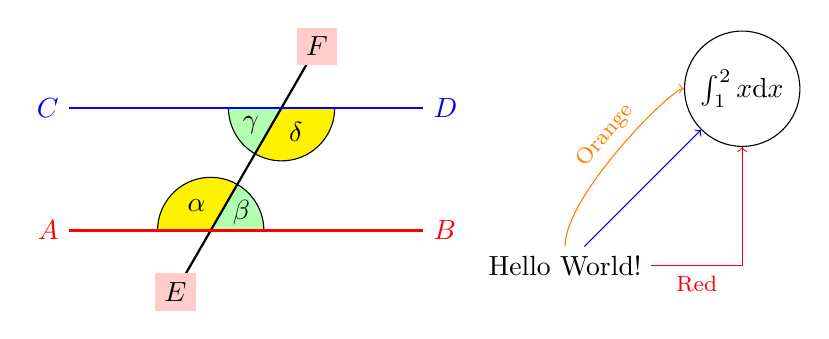
\begin{tikzpicture}[scale=0.9]
      \draw[fill=yellow] (0,0) -- (60:.75cm) arc (60:180:.75cm);
      \draw(120:0.4cm) node {$\alpha$};
      \draw[fill=green!30] (0,0) -- (right:.75cm) arc (0:60:.75cm);
      \draw(30:0.5cm) node {$\beta$};
      \begin{scope}[shift={(60:2cm)}]
        \draw[fill=green!30] (0,0) -- (180:.75cm) arc (180:240:.75cm);
        \draw (30:-0.5cm) node {$\gamma$};
        \draw[fill=yellow] (0,0) -- (240:.75cm) arc (240:360:.75cm);
        \draw (-60:0.4cm) node {$\delta$};
      \end{scope}
      \begin{scope}[thick]
        \draw (60:-1cm) node[fill=red!20] {$E$} -- (60:3cm) node[fill=red!20] {$F$};
        \draw[red] (-2,0) node[left] {$A$} -- (3,0) node[right]{$B$};
        \draw[blue,shift={(60:2cm)}] (-3,0) node[left] {$C$} -- (2,0) node[right]{$D$};
      \end{scope}
      \path (5,-0.5) node (x) {Hello World!}
      (7.5,2) node[circle,draw](y) {$\int_1^2 x \mathrm d x$};
      \draw[->,blue] (x) -- (y);
      \draw[->,red] (x) -| node[near start,below] {\footnotesize Red} (y);
      \draw[->,orange] (x) .. controls +(up:1cm) and +(left:1cm) .. node[above,sloped] {\footnotesize Orange} (y);
    \end{tikzpicture}

\end{frame}

\note{
  Example from J\"{o}rg Cassens, University of Trondheim, in his example:
  \vskip 1cm
  See \href{http://story.idi.ntnu.no/~cassens/blog/categories/20-LaTeX}{his blog on the Trondheim theme}.
}

\begin{frame}
  \frametitle{Using Ti\textit{k}Z for Petri-Net}
  \begin{center}
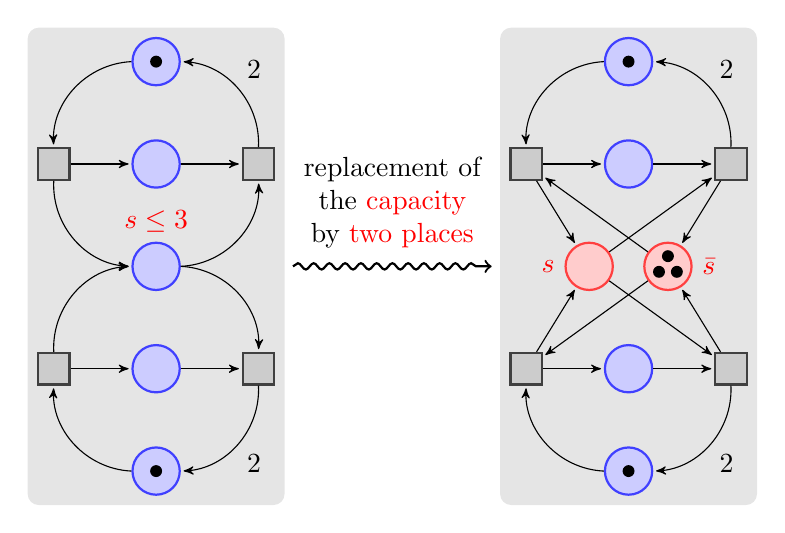
\begin{tikzpicture}
  [node distance=1.3cm,>=stealth',bend angle=45,auto,
   place/.style={circle,thick,draw=blue!75,fill=blue!20,minimum size=6mm},
   red place/.style={place,draw=red!75,fill=red!20},
   transition/.style={rectangle,thick,draw=black!75,fill=black!20,minimum size=4mm},
   every label/.style={red},on grid]

  \begin{scope}
    % First net
    \node [place,tokens=1] (w1)                                    {};
    \node [place] (c1) [below=of w1]                      {};
    \node [place] (s)  [below=of c1,label=above:$s\le 3$] {};
    \node [place] (c2) [below=of s]                       {};
    \node [place,tokens=1] (w2) [below=of c2]                      {};

    \node [transition] (e1) [left=of c1] {}
      edge [pre,bend left]                  (w1)
      edge [post,bend right]                (s)
      edge [post]                           (c1);

    \node [transition] (e2) [left=of c2] {}
      edge [pre,bend right]                 (w2)
      edge [post,bend left]                 (s)
      edge [post]                           (c2);

    \node [transition] (l1) [right=of c1] {}
      edge [pre]                            (c1)
      edge [pre,bend left]                  (s)
      edge [post,bend right] node[swap] {2} (w1);

    \node [transition] (l2) [right=of c2] {}
      edge [pre]                            (c2)
      edge [pre,bend right]                 (s)
      edge [post,bend left]  node {2}       (w2);
  \end{scope}

  \begin{scope}[xshift=6cm]
    % Second net
    \node [place,tokens=1]
                      (w1')                                                {};
    \node [place]     (c1') [below=of w1']                                 {};
    \node [red place] (s1') [below=of c1',xshift=-5mm,label=left:$s$]      {};
    \node [red place,tokens=3]
                      (s2') [below=of c1',xshift=5mm,label=right:$\bar s$] {};
    \node [place]     (c2') [below=of s1',xshift=5mm]                      {};
    \node [place,tokens=1]
                      (w2') [below=of c2']                                 {};

    \node [transition] (e1') [left=of c1'] {}
      edge [pre,bend left]                  (w1')
      edge [post]                           (s1')
      edge [pre]                            (s2')
      edge [post]                           (c1');

    \node [transition] (e2') [left=of c2'] {}
      edge [pre,bend right]                 (w2')
      edge [post]                           (s1')
      edge [pre]                            (s2')
      edge [post]                           (c2');

    \node [transition] (l1') [right=of c1'] {}
      edge [pre]                            (c1')
      edge [pre]                            (s1')
      edge [post]                           (s2')
      edge [post,bend right] node[swap] {2} (w1');

    \node [transition] (l2') [right=of c2'] {}
      edge [pre]                            (c2')
      edge [pre]                            (s1')
      edge [post]                           (s2')
      edge [post,bend left]  node {2}       (w2');
  \end{scope}

  \begin{pgfonlayer}{background}
    \node (r1) [fill=black!10,rounded corners,fit=(w1)(w2)(e1)(e2)(l1)(l2)] {};
    \node (r2) [fill=black!10,rounded corners,fit=(w1')(w2')(e1')(e2')(l1')(l2')] {};
  \end{pgfonlayer}

  \draw [shorten >=1mm,-to,thick,decorate,decoration={snake,amplitude=.4mm,segment
      length=2mm,pre=moveto,pre length=1mm,post length=2mm}]
    (r1) -- (r2)
    node [above=1mm,midway,text width=3cm,text centered]
      {replacement of the \textcolor{red}{capacity} by \textcolor{red}{two places}};

\end{tikzpicture}
  \end{center}
\end{frame}

%% PFG capabilities
% \begin{frame}
%   \frametitle{Using Ti\textit{k}Z for Drawings -- 2}

%   \begin{pgfpicture}{0cm}{0cm}{5cm}{2cm}
%     \pgfputat{\pgfxy(1,1)}{\pgfbox[center,center]{Hi!}}
%     \pgfcircle[stroke]{\pgfxy(1,1)}{0.5cm}
%     \pgfline{\pgfxy(1.5,1)}{\pgfxy(2.2,1)}
%      \pgfputat{\pgfxy(3,1)}{
%      \begin{pgfrotateby}{\pgfdegree{30}}
%        \pgfbox[center,center]{$\int_0^\infty xdx$}
%      \end{pgfrotateby}}
%     \pgfcircle[stroke]{\pgfxy(3,1)}{0.75cm}
%     \pgfmoveto{\pgfxy(5,1)}
%     \pgfcurveto{\pgfxy(6,0.5)}{\pgfxy(6,1.5)}{\pgfxy(8,1)}
%     \pgfstroke
%     \pgfsetdash{{3pt}{3pt}}{0pt}
%     \pgfmoveto{\pgfxy(5,1)}
%     \pgflineto{\pgfxy(6,0.5)}
%     \pgflineto{\pgfxy(6,1.5)}
%     \pgflineto{\pgfxy(7,1)}
%     \pgfstroke
%     \pgfmoveto{\pgfxy(9,1)}
%     \pgfcurveto{\pgfxy(9,0)}{\pgfxy(10,0)}{\pgfxy(10,1)}
%     \pgfcurveto{\pgfxy(10,2)}{\pgfxy(9,2)}{\pgfxy(9,1)}
%     \pgfclosepath
%     \pgffill
%   \end{pgfpicture}

% \end{frame}


% %% Movies capabilities
% \begin{frame}
%   \frametitle{Including Movies}

%   \pgfdeclareimage[interpolate=true,width=.45\textwidth]{ccpict}{Building_On_The_Past}

%   \begin{center}
%     \movie[poster,externalviewer,label=mymovie]{\pgfuseimage{mypic}}{mymovie_path.mpg}
%   \end{center}

%   {\small
%   To watch the movie in an external player application, click on the picture above.% or \hyperlinkmovie{mymovie}{\beamerbutton{press this button}}.

%   The video is not included in the distribution of this PDF. To watch it, just \href{http://some/long/path/to/the/file.mpg}{\alert{fix }names, paths and all}.

%   {\tiny Don't forget the copyright...}

% \end{frame}

\section{Benchmark Applications}

\subsection{Design}

\begin{frame}
  \frametitle{Applications}

  Different implementations

\end{frame}

\begin{frame}
  \frametitle{Learning Algorithm}

  Add the Algorithm

\end{frame}

\subsection{Development}

\begin{frame}
  \frametitle{C based HDR-NN}

  Add some code maybe

\end{frame}


\subsection{Results}

\begin{frame}
  \frametitle{Graphs}

  Figures

\end{frame}

\section{Discussion}

\begin{frame}[fragile]
  \frametitle{Development Experience}

  Development Experience

\end{frame}

\section{Conclusions}

\begin{frame}
  \frametitle{Conclusions}

%   \begin{itemize}
%     \item Non official
%     \item Suited for (long) scientific talks with UU style
%     \item The colours used in this theme are based on  ``UU red'' (and shades)
%     \item The hide[all|other]subsections switch is useful if you are having (too) many (sub-) sections
%     \item Several look \& feel options
%     \item Feedback appreciated: \href{mailto:daz@it.uu.se}{\texttt{daz@it.uu.se}}
%   \end{itemize}
\end{frame}

\end{document}
